%% abtex2-modelo-projeto-pesquisa.tex, v-1.9.6 laurocesar
%% Copyright 2012-2016 by abnTeX2 group at http://www.abntex.net.br/ 
%%
%% This work may be distributed and/or modified under the
%% conditions of the LaTeX Project Public License, either version 1.3
%% of this license or (at your option) any later version.
%% The latest version of this license is in
%%   http://www.latex-project.org/lppl.txt
%% and version 1.3 or later is part of all distributions of LaTeX
%% version 2005/12/01 or later.
%%
%% This work has the LPPL maintenance status `maintained'.
%% 
%% The Current Maintainer of this work is the abnTeX2 team, led
%% by Lauro César Araujo. Further information are available on 
%% http://www.abntex.net.br/
%%
%% This work consists of the files abntex2-modelo-projeto-pesquisa.tex
%% and abntex2-modelo-references.bib
%%

% ------------------------------------------------------------------------
% ------------------------------------------------------------------------
% abnTeX2: Modelo de Projeto de pesquisa em conformidade com 
% ABNT NBR 15287:2011 Informação e documentação - Projeto de pesquisa -
% Apresentação 
% ------------------------------------------------------------------------ 
% ------------------------------------------------------------------------

\documentclass[
	% -- opções da classe memoir --
	12pt,				% tamanho da fonte
 	openright,			% capítulos começam em pág ímpar (insere página vazia caso preciso)
 	oneside,
 	%twoside,			% para impressão em recto e verso. Oposto a oneside
	a4paper,			% tamanho do papel. 
	% -- opções da classe abntex2 --
	%chapter=TITLE,		% títulos de capítulos convertidos em letras maiúsculas
	%section=TITLE,		% títulos de seções convertidos em letras maiúsculas
	%subsection=TITLE,	% títulos de subseções convertidos em letras maiúsculas
	%subsubsection=TITLE,% títulos de subsubseções convertidos em letras maiúsculas
	% -- opções do pacote babel --
	english,			% idioma adicional para hifenização
	french,				% idioma adicional para hifenização
	spanish,			% idioma adicional para hifenização
	brazil,				% o último idioma é o principal do documento
	]{abntex2}

% ---
% PACOTES
% ---

% ---
% Pacotes fundamentais 
% ---
\usepackage{lmodern}			% Usa a fonte Latin Modern
\usepackage[T1]{fontenc}		% Selecao de codigos de fonte.
\usepackage[utf8]{inputenc}		% Codificacao do documento (conversão automática dos acentos)
\usepackage{indentfirst}		% Indenta o primeiro parágrafo de cada seção.
\usepackage{color}				% Controle das cores
\usepackage{graphicx}			% Inclusão de gráficos
\usepackage{microtype} 			% para melhorias de justificação
% ---

% ---
% Pacotes adicionais, usados apenas no âmbito do Modelo Canônico do abnteX2
% ---
\usepackage{lipsum}				% para geração de dummy text
% ---
\usepackage[brazil]{babel}
\usepackage{listings}
\usepackage{color}		

% ---
% Pacotes de citações
% ---
\usepackage[brazilian,hyperpageref]{backref}	 % Paginas com as citações na bibl
\usepackage[alf]{abntex2cite}	% Citações padrão ABNT

% --- 
% CONFIGURAÇÕES DE PACOTES
% --- 

% ---
% Configurações do pacote backref
% Usado sem a opção hyperpageref de backref
\renewcommand{\backrefpagesname}{Citado na(s) página(s):~}
% Texto padrão antes do número das páginas
\renewcommand{\backref}{}
% Define os textos da citação
\renewcommand*{\backrefalt}[4]{
	\ifcase #1 %
		Nenhuma citação no texto.%
	\or
		Citado na página #2.%
	\else
		Citado #1 vezes nas páginas #2.%
	\fi}%
% ---

% ---
% Informações de dados para CAPA e FOLHA DE ROSTO
% ---
\titulo{Wiring, Arduíno e AVR. Como estas tecnologias estão associadas}
\autor{Ricardo Aparecido Bezerra Elias da Silva - 15203158\\Renato Frutuoso - 15101598\\Robson Araújo - 33001136\\Lucas Rafael 15203792}
\local{Osasco}
\data{2018}
\instituicao{%
  Centro Universitário UNIFIEO
  \par
  Engenharia da Computação
  \par
  Engenharia de Software II}
\tipotrabalho{Tese (Doutorado)}
% O preambulo deve conter o tipo do trabalho, o objetivo, 
% o nome da instituição e a área de concentração 
\preambulo{Pesquisa referente a disciplina de Laboratório Integrado II, Prof. Bruno Abrantis, sobre a relação entre Wiring e o Arduíno e como estas tecnologias utilizam o microcontrolador AVRs.}
% ---

% ---
% Configurações de aparência do PDF final

% alterando o aspecto da cor azul
\definecolor{blue}{RGB}{41,5,195}

% informações do PDF
\makeatletter
\hypersetup{
     	%pagebackref=true,
		pdftitle={\@title}, 
		pdfauthor={\@author},
    	pdfsubject={\imprimirpreambulo},
	    pdfcreator={LaTeX with abnTeX2},
		pdfkeywords={abnt}{latex}{abntex}{abntex2}{projeto de pesquisa}, 
		colorlinks=true,       		% false: boxed links; true: colored links
    	linkcolor=blue,          	% color of internal links
    	citecolor=blue,        		% color of links to bibliography
    	filecolor=magenta,      		% color of file links
		urlcolor=blue,
		bookmarksdepth=4
}
\makeatother
% --- 

% --- 
% Espaçamentos entre linhas e parágrafos 
% --- 

% O tamanho do parágrafo é dado por:
\setlength{\parindent}{1.3cm}

% Controle do espaçamento entre um parágrafo e outro:
\setlength{\parskip}{0.2cm}  % tente também \onelineskip

% ---
% compila o indice
% ---
\makeindex
% ---

% ----
% Início do documento
% ----
\begin{document}

% Seleciona o idioma do documento (conforme pacotes do babel)
%\selectlanguage{english}
\selectlanguage{brazil}

% Retira espaço extra obsoleto entre as frases.
\frenchspacing 

% ----------------------------------------------------------
% ELEMENTOS PRÉ-TEXTUAIS
% ----------------------------------------------------------
% \pretextual

% ---
% Capa
% ---
\imprimircapa
% ---

% ---
% Folha de rosto
% ---
\imprimirfolhaderosto
% ---

% ---
% NOTA DA ABNT NBR 15287:2011, p. 4:
%  ``Se exigido pela entidade, apresentar os dados curriculares do autor em
%     folha ou página distinta após a folha de rosto.''
% ---
\setlength{\absparsep}{18pt} % ajusta o espaçamento dos parágrafos do resumo
\begin{resumo}
    O hardware open-source Arduíno está de fato consolidado no mundo da eletrônica. A facilidade em manuseá-lo e a sua aplicabilidade fazem com que o ensino de robôtico e programação cresça cada vez mais em todo o mundo. É importante citar que o sucesso do Arduíno tem mais de um protagonista: Wiring, Process e AVR. Nesta pesquisa falamos um pouco sobre cada uma destas tecnologias como suas histórias se cruzam. Apresentamos também as bibliotecas que linkan estas tecnologias e mostramos a definição de algumas funções que são muito utilizadas no início da aprendizagem de Arduíno.

 \textbf{Palavras-chave}: wiring. arduino. process, hardware.
\end{resumo}
% ---
% inserir lista de ilustrações
% ---
% \pdfbookmark[0]{\listfigurename}{lof}
% \listoffigures*
% \cleardoublepage
% ---

% ---
% inserir lista de tabelas
% ---
% \pdfbookmark[0]{\listtablename}{lot}
% \listoftables*
% \cleardoublepage
% ---

% ---
% inserir lista de abreviaturas e siglas
% ---
%\begin{siglas}
%  \item[ABNT] Associação Brasileira de Normas Técnicas
%  \item[abnTeX] ABsurdas Normas para TeX
%\end{siglas}
% ---

% ---
% inserir lista de símbolos
% ---
%\begin{simbolos}
%  \item[$ \Gamma $] Letra grega Gama
%  \item[$ \Lambda $] Lambda
%  \item[$ \zeta $] Letra grega minúscula zeta
%  \item[$ \in $] Pertence
%\end{simbolos}
% ---

% ---
% inserir o sumario
% ---
\pdfbookmark[0]{\contentsname}{toc}
\tableofcontents*
\cleardoublepage
% ---


% ----------------------------------------------------------
% ELEMENTOS TEXTUAIS
% ----------------------------------------------------------
\textual

% ----------------------------------------------------------
% Introdução
% ----------------------------------------------------------
\section[Wiring]{Wiring}

\subsection{Início do Wiring}
Barragán, um dos criadores do Wiring, define sua criação como "um ambiente de programação e uma placa de entrada / saída de prototipagem eletrônica para explorar as artes eletrônicas e a mídia tangível"\cite{Barragan2004}.

O projeto Wiring foi iniciado em 2003 durante o mestrado de Barragán pela Interaction Design Institute Ivrea (IDII), Italia \footnote{\url{http://wiki.wiring.co/wiki/About}}. Sua idéia era disponibilizar a designers e artistas uma plataforma eletrônica de fácil utilização, retirando a necessidade de estudo afundo em linguagens de programação e eletrônica fazendo o usuário ter maior foco no que de fato é sua expertise. Esta facilidade também poderia ser aplicada no ensino de programação e prototipagem nas escolas.

Barragán se formou com distinção, o único a conseguir tal fação na IDII em 2004.

No outono do mesmo ano, o Wiring foi utilizado em curso de inverno de computação física na IDII, sendo o nome do projeto Stranger Familiar, ministrado por nomes como Massimo Banzi, Heather Martin, Yaniv Steiner, Reto Wettach. Neste projeto foi proposto a criação de objetos domésticos incomuns porém interessantíssimos\footnote{\url{http://wiring.org.co/exhibition/images/book01.pdf}}

\subsection{Wiring e o Processing}

O Processing foi criado em 2001 por Ben Fry e Casey Reas. Seu objetivo era tornar a programação mais visual, facilitando a entrada de não-programadores ao meio da computação, principalmente voltado a artes e design.\cite{reas2007processing} A linguagem tem por base as capacidades gráficas da linguagem de programação Java. O Wiring foi desenvolvido através do Processing.

"Processing, como um subconjunto na linguagem Java, traz aos usuários uma interface de aplicativo independente da tecnologia na qual ele é usado, mantendo um nível de abstração que permite aos usuários aprender os fundamentos da programação de computadores e se concentrar em seus projetos ao invés de questões ou especificidades tecnológicas de uma plataforma. A linguagem de programação Java oferece uma sintaxe muito semelhante a C, C ++, Javascript ou Flash Actionscript, possibilitando a construção de programas e algoritmos que podem ser facilmente traduzidos para diferentes linguagens e ambientes. Isso faz do Processing uma ferramenta muito interessante para ensinar e aprender programação de computadores."\cite{Barragan2004}.

\subsection{Wiring e o Arduíno}

Ao contrário da relação entre Wiring e Processing, há uma grande discussão sobre o reconhecimento de o Arduíno ser uma derivação do Wiring.
Na página de créditos do Arduíno \footnote{\url{http://wiki.wiring.co/wiki/About}}, os autores informam que o Arduíno "(...)deriva do Wiring, uma plataforma construída por Hernando Barragán como sua tese de mestrado na Interaction-Ivrea" mas reforçam que o Wiring e, por sua vez, o Arduíno são derivados de um projeto chamado Massimo's Programma2003 (Figura \ref{programma2003}) e Processing, o último reconhecido por Barragán. 

\begin{figure}[htb]
	\caption{\label{programma2003}Placa Programma2003 projetada por Massimo Banzi em 2003}
	\begin{center}
	    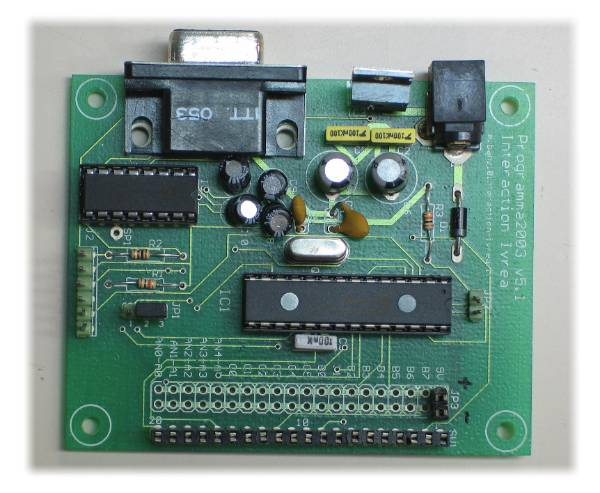
\includegraphics[scale=0.3]{refs/Programma2003}
	\end{center}
	%\legend{Fonte: Site da 3GPP}
\end{figure}

Já o criador do Wiring, criou uma página de nome "The Untold History of Arduino" \footnote{\url{https://arduinohistory.github.io/}} onde explica, em tom de crítica, diversos tópicos sobre o Arduíno.

%https://arduinohistory.github.io/
%http://wiki.wiring.co/wiki/About
%http://wiring.org.co/exhibition/images/book01.pdf
%https://www.arduino.cc/en/Main/Credits
\section[O Hardware]{O Hardware}

O hardware Wiring (\autoref{wiringS}) é uma pequena placa de circuito com um microcontrolador atmega644p, construída com base na linguagem Processing. Abaixo algumas características básicas desta placa: 

\begin{alineas}
    \item Pinos digitais de entrada e saída
    \item Pino analógico de entrada
    \item Pino PWM\footnote{\url{https://www.citisystems.com.br/pwm/}} de saída
    \item Porta serial (disponível através do conector USB)
    \item Fonte de alimentação de 7 a 12 Volts
\end{alineas}

Possui aplicações em ensino de eletrônica, ensino de programação de computadores, mídia tangível, arte interativa, etc.

Para mais características consultar o site do fabricante\footnote{\url{http://wiring.org.co/hardware/}}

\begin{figure}[htb]
	\caption{\label{wiringS}Placa Wiring S}
	\begin{center}
	    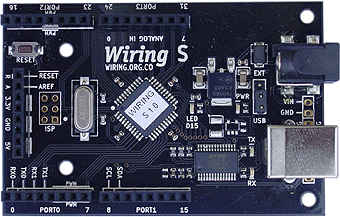
\includegraphics[scale=0.9]{artigo/refs/Rogue_BB_WRS}
	\end{center}
	%\legend{Fonte: Site da 3GPP}
\end{figure}
\section{Software Wiring}

% Verificar na própria tese do Barragàn os Tópicos 4 e 5. Já dá para adiantar que não será assunto suficiente, então será necessário dar uma pequena pesquisada. Não precisa ser longo o conteúdo
\section{A biblioteca Wiring no Arduíno}
\subsection{Principais Funções}
\chapter{Wiring e o AVR}

\section{Atmel AVR}

O AVR é um microcontrolador RISC desenvolvido pela Atmel e posteriormente comprado pela Microchip Tecnology. Possui uma pequena memória flash para armazenamento do programas e 32 registradores internos. Este tipo de chip é muito utilizado em hardwares de prototipagem, como o Arduíno.

Conforme \citeonline{borges2006desenvolvimento} "Com o objetivo de maximizar o desempenho e o paralelismo, o AVR segue arquitetura Harvard, em que os barramentos associados às memórias de dados e do programa são distintos. Além disso, utiliza-se a técnica do \emph{pipeline}, em que, enquanto uma instrução começa a ser executada, uma outra já é buscada na memória de programa para que a mesma possa ser executada no próximo ciclo de relógio"

Um microcontrolador possui internamente todas as caracteristicas de um computador possuindo processador, memória e periféricos de entrada e saída. Este tipo de circuito é conhecido como \emph{System-on-chip}. Esta característica o faz ser amplamente utilizado em hardwares de prototipagem pois possui características suficientes para a execução de programas e acionamento de pinos, por exemplo.

A versão mais popular do Arduíno, o Arduíno Uno, possui um microcontrolador ATmega328 (\autoref{atmega})

\begin{figure}[htb]
	\begin{center}
	    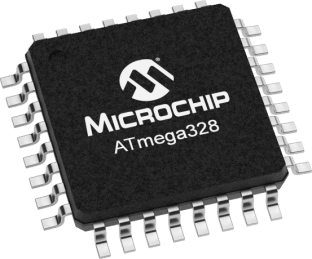
\includegraphics[scale=0.5]{artigo/refs/medium-ATmega328-TQFP-32.png}
	\end{center}
	\caption{\label{atmega}chip ATmega328}
	%\legend{Fonte: Site da 3GPP}
\end{figure}

Algumas das características do ATmega328 são listadas na tabela abaixo

\section{Programando para AVR}

No diretório de instalação do Arduíno há uma biblioteca denominada avr/io.h, esta biblioteca possui todas as diretivas para outras bibliotecas com base no microcontrolador utilizado. Nestas bibliotecas há definições de registradores de entrada e saída, pinos, constantes e diversos outros componentes, conforme trecho abaixo.

\subsection{Bibliotecas AVR}

Aqui um pequno trecho da biblioteca io.h em que, de acordo com o chip AVR utilizado, uma nova biblioteca é incluída.
\newline
\newline
\begin{lstlisting}
//biblioteca io.h
//(...)
#ifndef _AVR_IO_H_
#define _AVR_IO_H_

#include <avr/sfr_defs.h>

#if defined (__AVR_AT94K__)
#  include <avr/ioat94k.h>
//(...)
#elif defined (__AVR_ATmega328P__)
#  include <avr/iom328p.h>
#elif (defined __AVR_ATmega328__)
#include <avr/iom328.h>
//(...)

\end{lstlisting}
%INSERIR IMAGEM DO ATMEGA328, INSERIR TAMBÉM UM TRECHO OU OUTRO E FINALIZAR

Aqui um pequno trecho da biblioteca io.h em que, de acordo com o chip AVR utilizado, uma nova biblioteca é incluída.

\begin{lstlisting}
//biblioteca iom328p.h
//(...)
#ifndef _AVR_IOM328P_H_
#define _AVR_IOM328P_H_ 1

/* Registers and associated bit numbers */

#define PINB _SFR_IO8(0x03)
#define PINB0 0
//(...)
#define DDRB _SFR_IO8(0x04)
#define DDB0 0
#define DDB1 1
//(...)
#define PORTB _SFR_IO8(0x05)
#define PORTB0 0
#define PORTB1 1
//(...)
\end{lstlisting}

\section{Conclusão}


% ---
% Finaliza a parte no bookmark do PDF
% para que se inicie o bookmark na raiz
% e adiciona espaço de parte no Sumário
% ---
\phantompart

% ---
% Conclusão
% ---
% ----------------------------------------------------------
% ELEMENTOS PÓS-TEXTUAIS
% ----------------------------------------------------------
\postextual

% ----------------------------------------------------------
% Referências bibliográficas
% ----------------------------------------------------------
\bibliography{refs/refs.bib}

% ----------------------------------------------------------
% Glossário
% ----------------------------------------------------------
%
% Consulte o manual da classe abntex2 para orientações sobre o glossário.
%
%\glossary

% ----------------------------------------------------------
% Apêndices
% ----------------------------------------------------------

% ---
% Inicia os apêndices
% ---
%\begin{apendicesenv}

% Imprime uma página indicando o início dos apêndices
%\partapendices


%\end{apendicesenv}
% ---


% ----------------------------------------------------------
% Anexos
% ----------------------------------------------------------

% ---
% Inicia os anexos
% ---
%\begin{anexosenv}

% Imprime uma página indicando o início dos anexos
%\partanexos

%\end{anexosenv}

%---------------------------------------------------------------------
% INDICE REMISSIVO
%---------------------------------------------------------------------

\phantompart

\printindex

\end{document}
